\documentclass{article}
\usepackage{blindtext}
\usepackage[a4paper, total={6in, 8in}]{geometry}
\usepackage{amsmath}
\usepackage{ amssymb }
\usepackage{cancel}
\usepackage{multirow}

\usepackage[inline]{asymptote}
\begin{asydef}
//
// Global Asymptote definitions can be put here.
//
usepackage("bm");
texpreamble("\def\V#1{\bm{#1}}");
\end{asydef}
\title{Abstract Algebra in the AMC!?}
\author{Eric Yee}
\date{November 2023}

\begin{document}

\maketitle

I always wished the AMC could test Abstract Algebra. I mean, who wouldn't? Thats why I went into Google and searched abstract algebra on the AMC, and amazingly I found something. Does this terrify you? That you might be the next unsuspecting victim of an abstract algebra problem on the AMC? Well, you are right to be scared. You should be TERREFIED. But don't worry, your salvation is in front of you. This article we will explain to you the magic and the terror of Burnsides Lemma.

Before we see it written out, we must identify some notation and concepts. First, we introduce the notion of a group. This concept deserves its own article (and a lot more), but a simple definition is that it is a set of elements with a \textbf{binary operation}, such that there exists an \textbf{identity}, is \textbf{invertible}, and is \textbf{associative}. Writing this out, this means if $G$ is a group, then there is a function $\times: G\oplus G \rightarrow G$, ie. $\forall g,h\in G$, there exists $f\in G$ such that $g\times h = f$. The other properties mean (identity) there exists $e\in G$, such that $\forall g\in G$, $e\times g=g\times e = g$, (invertible) $\forall g\in G$, there exists $h\in G$ such that $gh=e$ and (associative) $\forall g,h,f\in G$, $(g\times h)\times f =g\times (h\times f)$.

A common example of a group is the set of integers under addition since taking the $0$ is your identity, negation is your inverse, and obviously, addition is associative.

Alright, but we are not done yet, we also need to define a \textbf{Group Action.} A group action is when we consider a group $G$ as a function that acts on a set $X$. This means that $\forall g\in G$, $g: X\rightarrow X$, ie. $\forall x\in X$ and $g\in G$, $g(x)\in X$. Moreover, these group actions also have to follow their binary operation under composition. So we have that $g(h(x)) = (gh)(x)$. 

One example of a $G$-action is if we take $G=\{R_0,R_{90},R_{180},R_{270}\}$  where $R_i$ is a clockwise rotation on the $xy$ plane by $i$ degrees, and the binary operation is composition, so $R_i \circ R_j = R_{i+j}.$ Then we can take $X$ to be the vertices of the cube. Then $R_{180}(5)=7$ and $R_{270}(1)=4$
\begin{center}
    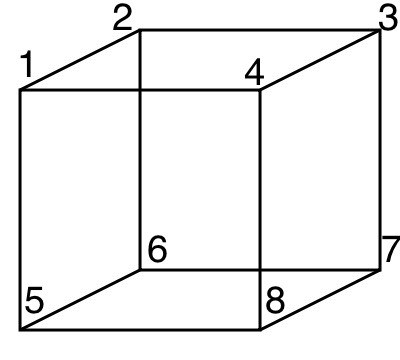
\includegraphics[width=8cm, scale=1]{nov23/images/Labeled_cube_graph.png}
\end{center}


We also have to identify what Orbits are. We'll define $O_x$ as the orbit of $x\in X$, which is basically where the element $x$ can go once you take $x$ as the function of an element of $G$ - hence the name. Formally, we have $O_x=\{y\in X | \exists g\in G, g(x)=y\}.$ Kind of the opposite, we also define $X^g$ as the elements in $X$ which are fixed by $g$, ie. $g(x) = x$.

Ok, we are almost there. To understand the lemma, we first have to see a fact about orbits. This is that they collectively partition the set $X$. To see why this is true, consider the example from before when $X$ was the vertices of a cube, and $G=\{R_0,R_{90},R_{180},R_{270}\}$. Here we see that each point on the lower face can be sent to every other point on the lower face but no other points. Similarly, the top points can be sent to each other but nowhere else. Thus the two orbits partition the total set of $8$ vertices into the $4$ vertices on the top face and $4$ on the bottom face.

Finally, here comes the lemma: If there is a group action on $X$ by the group $G$, then the number of distinct orbits is $$\frac{1}{|G|}\sum_{g\in G}|X^g|,$$
or in other words, the number of distinct orbits is the average size of the number of elements stabilized by an element of $G$.

I know, it looks kinda scary, but let's see it in action, with, as promised, an AMC problem:

Problem 13 AMC 12B 2017:
In the figure below, $3$ of the $6$ disks are to be painted blue, $2$ are to be painted red, and $1$ is to be painted green. Two paintings that can be obtained from one another by a rotation or a reflection of the entire figure are considered the same. How many different paintings are possible?
\begin{center}
    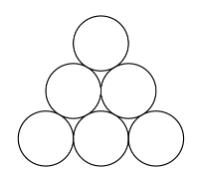
\includegraphics[width=10cm, scale=1.5]{nov23/images/amc12b1017p13.png}
\end{center}

$\textbf{(A) } 6 \qquad \textbf{(B) } 8 \qquad \textbf{(C) } 9 \qquad \textbf{(D) } 12 \qquad \textbf{(E) } 15$

Let's rewrite the problem in terms of Burnsides Lemma. In this case, the group action is rotations and reflections, so specifically our group is $D_3=\{R_0,R_{120},R_{240}, I,V,W\}$ where $R_i$ is a rotation by $i$ degrees and $I, V, W$ is reflecting vertically, North West to South East, and North East to South West respectively. It can be verified that $G$ is a group if we take the binary operation to be composition.

Now we take our set $X$ to be the total number of diagrams. Then the question is asking for the number of distinct orbits under $D_3$, since $D_3$ accounts for the rotations and reflections. This we know is 
$$\frac{1}{|D_3|}\sum_{g\in D_3}|X^g|,$$
so all we need to do is find the number of diagrams that are stable under each element of $D_3$. Lets number the circles as following so we can easily reference them:
\begin{center}
    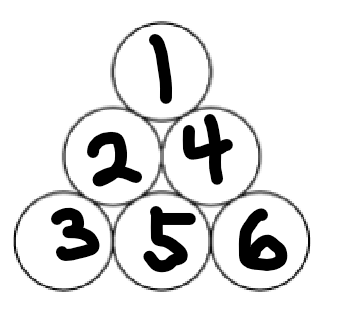
\includegraphics[width=10cm, scale=1.5]{nov23/images/modifiedamcimage.png}
\end{center}
If $g=R_0$, then every disk is disk is unaffected, so all diagrams are fixed. Thus $|X^{R_0}|=\binom{6}{3}\binom{3}{2}=60$. 

If $g=R_{120}$, then we can see no disk is fixed, so if we want $R_{120}$ to stabilize the diagram, then it must be that the colors of $1,6,3$ and $4,5,2$ are the same. This is impossible so $|X^{R_{120}}|=0$.

If $g=R_{240}$, then its the same thing so $|X^{R_{240}}|=0$.

If $g=I$, then $1$ and $5$ are fixed, but if we want $I$ to stabilize a diagram, then the colors of $2,4$ and $3,6$ must be the same. The only configuration that works is if $1$ or $5$ is green and the other is blue, $2,4$ is blue or red, and $3,6$ is the one $2,4$ was not. In total $|X^{I}| = 2\cdot 2 =4.$

The cases where $g=V$ and $g=W$ are the same as $g=I$. Thus in total, we have

\begin{align*}
    \frac{1}{|D_3|}\sum_{g\in D_3}|X^g| &= \frac{60+0+0+4+4+4}{6}\\
    &=\boxed{\text{D: }12}.
\end{align*}

We did it! We corrupted the AMC with Abstract Algebra! This shows that no matter how you try to hide from it, Abstract Algebra will always creep up on you. Who knows, maybe Burnsides Lemma will appear on the AMC next year, but now you'll be ready.
\end{document}
In this way (for those of you who know what a homomorphism is), a group action is really just homomorphism from $(G,\times)$ into the group of possible transformations on $X$.